\documentclass[11pt,a4paper]{article}

% --- Packages ------------------------------------------------------------
\usepackage[T1]{fontenc}
\usepackage[utf8]{inputenc}
\usepackage[english]{babel}
\usepackage{amsmath,amssymb,amsthm}
\usepackage{geometry}
\usepackage{hyperref}
\usepackage{xcolor}
\usepackage{listings}
\usepackage{booktabs}
\usepackage{array}
\usepackage{graphicx}
\usepackage[activate=false]{microtype}
\usepackage{parskip}
\usepackage{enumitem}
\usepackage{titlesec}
\usepackage{fancyhdr}
\usepackage{natbib}

\geometry{margin=2.5cm, top=3cm, bottom=3cm}

% --- Colours ------------------------------------------------------------
\definecolor{juliaBlue}{RGB}{64,99,216}
\definecolor{juliaGreen}{RGB}{28,161,83}
\definecolor{juliaRed}{RGB}{203,60,51}
\definecolor{juliaPurple}{RGB}{149,88,178}
\definecolor{codeGray}{RGB}{248,248,248}
\definecolor{commentGray}{RGB}{130,130,130}
\definecolor{stringGreen}{RGB}{0,128,0}

% --- Listings ------------------------------------------------------------
\lstdefinelanguage{Julia}{
  keywords={function,end,return,if,else,elseif,for,while,in,
            using,import,export,module,struct,mutable,abstract,
            where,begin,let,do,try,catch,finally,nothing,true,false},
  keywordstyle=\color{juliaBlue}\bfseries,
  sensitive=true,
  comment=[l]{\#},
  commentstyle=\color{commentGray}\itshape,
  stringstyle=\color{stringGreen},
  morestring=[b]",
  morestring=[b]',
}

\lstset{
  language=Julia,
  backgroundcolor=\color{codeGray},
  basicstyle=\ttfamily\small,
  breaklines=true,
  breakatwhitespace=true,
  frame=single,
  framesep=4pt,
  rulecolor=\color{gray!40},
  xleftmargin=8pt,
  xrightmargin=8pt,
  numbers=none,
  showstringspaces=false,
  tabsize=4,
}

% --- Theorem environments ------------------------------------------------------
\theoremstyle{definition}
\newtheorem{definition}{Definition}[section]
\newtheorem{remark}{Remark}[section]

% --- Headers / footers --------------------------------------------------------
\pagestyle{fancy}
\fancyhf{}
\fancyhead[L]{\small\textsc{RiemannBasins.jl — User Manual}}
\fancyhead[R]{\small\thepage}
\renewcommand{\headrulewidth}{0.4pt}

% --- Macros ------------------------------------------------------------
\newcommand{\C}{\mathbb{C}}
\newcommand{\R}{\mathbb{R}}
\newcommand{\Pone}{\mathbb{P}^1(\C)}
\newcommand{\Ptwo}{\mathbb{P}^1_+(\C)}
\newcommand{\pkg}[1]{\texttt{#1}}
\newcommand{\fn}[1]{\texttt{#1}}
\newcommand{\kw}[1]{\texttt{\textbf{#1}}}
\newcommand{\opt}[1]{\texttt{#1}}

% --- Title ------------------------------------------------------------
\title{%
  \vspace{-1cm}
  {\Large \textbf{RiemannBasins.jl}}\\[4pt]
  {\large Basin Portraits on the Riemann Sphere}\\[6pt]
  {\normalsize User Manual — Version 1.0}
}
\author{%
  Luis Javier Hernández Hernández\\
  \small Departamento de Matemáticas y Computación\\
  \small Universidad de La Rioja\\
  \small \href{mailto:luis-javier.hernandez@unirioja.es}{luis-javier.hernandez@unirioja.es}
}
\date{October 2026}

% ------------------------------------------------------------
\begin{document}
% ------------------------------------------------------------

\maketitle
\thispagestyle{empty}

\begin{abstract}
\pkg{RiemannBasins.jl} is a Julia package for visualising the basins of attraction
of discrete semi-flows induced by iterating univariate rational functions on
the Riemann sphere $\Pone$.
It supports standard and colour-blind-safe rendering, smooth colouring with
cyclic banding, two-chart (projective) plots, GIF animations of parametric
families, and three-dimensional basin-relief surfaces that display fractal
texture as a low-relief embossing of the convergence landscape.
This manual describes the mathematical background, the public API, and
includes worked examples.
\end{abstract}

\tableofcontents
\newpage

% ------------------------------------------------------------
\section{Introduction}
% ------------------------------------------------------------

Iterating a rational function $f:\Pone\to\Pone$ partitions the sphere into
\emph{basins of attraction}: the set of all points that converge to a given
fixed point (or periodic orbit) under repeated application of $f$.
These basins are the dynamical counterpart of the Newton fractal, which
corresponds to the specific choice $f = N_p$ (Newton's method for a
polynomial $p$).

Visualising basins reveals the fractal geometry of the Julia set — the
boundary separating distinct basins — and is a standard tool in complex
dynamics \citep{milnor2006,beardon1991}.

\pkg{RiemannBasins.jl} automates the complete pipeline:

\begin{enumerate}[nosep]
  \item Computing the homogeneous representation of the rational function.
  \item Finding all finite fixed points.
  \item Iterating each pixel of a rectangular grid until convergence.
  \item Rendering the result with one of three colour strategies,
        including smooth colouring and cyclic banding.
  \item Producing plots in the affine chart, the two-chart atlas,
        or as an animated GIF.
\end{enumerate}

% ------------------------------------------------------------
\section{Mathematical Background}
% ------------------------------------------------------------

\subsection{The projective line $\Pone$}

The complex projective line $\Pone$ consists of equivalence classes
$[z_0 : z_1]$ of pairs $(z_0, z_1) \in \C^2 \setminus \{(0,0)\}$, where
$(z_0,z_1)\sim(\lambda z_0,\lambda z_1)$ for every $\lambda\in\C^*$.
It is homeomorphic to the Riemann sphere $S^2$.

The affine chart $z_1\ne 0$ identifies $[z_0:z_1]$ with $z = z_0/z_1\in\C$;
the remaining point $[1:0]$ corresponds to $\infty$.

\pkg{RiemannBasins.jl} represents points as \emph{homogeneous pairs}
$(z_0,z_1)\in\C^2$, normalised so that
\[
  \max(|z_0|,|z_1|) = 1,
\]
and appends a \emph{super-zero} absorbing state $(0,0)$ to handle
computational indeterminations, yielding the augmented space
$\Ptwo = \Pone \cup \{[0:0]\}$.

\subsection{Chordal metric}

The \emph{chordal metric} on $\Pone$ between two points
$P=[z_0:z_1]$ and $Q=[w_0:w_1]$ (normalised) is
\[
  \chi(P,Q)
  = \frac{|z_0 w_1 - z_1 w_0|}%
         {\sqrt{|z_0|^2+|z_1|^2}\,\sqrt{|w_0|^2+|w_1|^2}}.
\]
It agrees with the Euclidean metric on the unit sphere in $\R^3$ under
stereographic projection and is bounded by $1$.

\subsection{Rational functions as homogeneous maps}

A rational function of degree $d$ is written $f = p/q$ where
$p,q\in\C[z]$ are coprime polynomials.
In homogeneous coordinates $[z_0:z_1]$ it lifts to
\[
  F(z_0,z_1) = \bigl[P(z_0,z_1)\;:\;Q(z_0,z_1)\bigr],
\]
where $P,Q\in\C[z_0,z_1]$ are the homogenisations of $p,q$:
\[
  P(z_0,z_1) = z_1^d\,p(z_0/z_1),\quad
  Q(z_0,z_1) = z_1^d\,q(z_0/z_1).
\]

\pkg{RiemannBasins.jl} stores a rational function as the pair of bivariate
polynomials $(P,Q)$ and evaluates it in homogeneous coordinates to avoid
division-by-zero issues near poles.

\subsection{Fixed points and basins}

A \emph{fixed point} of $f$ is a point $w\in\Pone$ such that $f(w)=w$.
For $f = p/q$ (degree $d$), there are at most $d+1$ fixed points on $\Pone$
(counted with multiplicity).

The \emph{basin of attraction} of a fixed point $w^*$ is
\[
  \mathcal{B}(w^*) = \bigl\{z\in\Pone : f^n(z)\to w^*\text{ as }n\to\infty\bigr\}.
\]
The \emph{Julia set} $\mathcal{J}(f)$ is the complement of the union of all
Fatou components; it coincides with $\partial\mathcal{B}(w^*)$ whenever the
latter is a basin.

\subsection{Newton's method as an example}

For the polynomial $p(z) = z^3 - 1$, Newton's method gives
\[
  N(z) = z - \frac{p(z)}{p'(z)} = z - \frac{z^3-1}{3z^2} = \frac{2z^3+1}{3z^2}.
\]
In homogeneous coordinates with the coefficient convention of
\pkg{RiemannBasins.jl} (constant term first):
\begin{lstlisting}
num = complex([1.0, 0.0, 0.0, 2.0])   # 1 + 0z + 0z^2 + 2z^3
den = complex([0.0, 0.0, 3.0, 0.0])   # 0 + 0z + 3z^2 + 0z^3
\end{lstlisting}
This gives $f(z) = (2z^3+1)/(3z^2)$, which has three fixed points at the
cube roots of unity $1,\,\omega,\,\omega^2$ with $\omega = e^{2\pi i/3}$.

% ------------------------------------------------------------
\section{Installation}
% ------------------------------------------------------------

\pkg{RiemannBasins.jl} requires Julia 1.9 or later.
It depends on the registered packages
\pkg{Polynomials.jl} (v3+), \pkg{Colors.jl}, and \pkg{Plots.jl}.

\paragraph{From a local clone (development mode)}
\begin{lstlisting}
# In the Julia REPL, activate the package environment:
using Pkg
Pkg.activate("path/to/RiemannBasins")
Pkg.instantiate()
using RiemannBasins
\end{lstlisting}

\paragraph{From the package directory}
\begin{lstlisting}
# From the operating system shell:
julia --project=path/to/RiemannBasins

# Inside the REPL:
using RiemannBasins
\end{lstlisting}

% ------------------------------------------------------------
\section{Quick Start}
% ------------------------------------------------------------

The following session produces Figure~\ref{fig:quickstart}: the basin portrait
of Newton's method for $z^3-1$ with smooth colouring and cyclic banding.

\begin{lstlisting}
using Pkg; Pkg.activate(".")
using RiemannBasins, Colors

# Newton's method for z^3 - 1
# Coefficient convention: constant term first
num = complex([1.0, 0.0, 0.0, 2.0])   # 2z^3 + 1
den = complex([0.0, 0.0, 3.0, 0.0])   # 3z^2

plt = basin_portrait(
    num, den;
    xinterval = (-1.5, 1.5),
    yinterval = (-1.5, 1.5),
    iter      = 200,
    colorstrategy = "positionplusiteration")
\end{lstlisting}

\begin{figure}[ht]
  \centering
  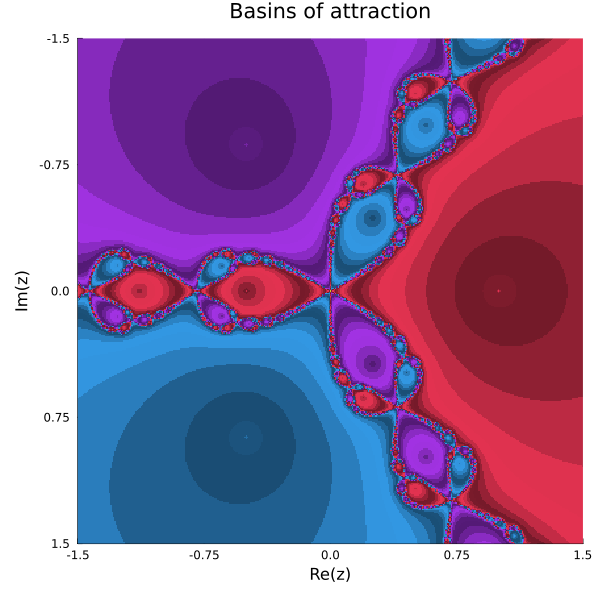
\includegraphics[width=0.55\textwidth]{figures/newton_z3_test.png}
  \caption{Basin portrait of Newton's method for $z^3-1$.
    Three basins (red, green, blue) separated by the Newton fractal.
    Cyclic banding reveals the convergence speed.}
  \label{fig:quickstart}
\end{figure}

% ------------------------------------------------------------
\section{Coefficient Convention}
% ------------------------------------------------------------

\pkg{RiemannBasins.jl} follows the same convention as \pkg{Polynomials.jl}:
coefficients are listed from \emph{lowest} to \emph{highest} degree.
Concretely, the vector \texttt{[c0, c1, c2, \ldots, cn]} represents
\[
  c_0 + c_1 z + c_2 z^2 + \cdots + c_n z^n.
\]

\begin{center}
\begin{tabular}{lll}
\toprule
Mathematical expression & Coefficient vector & Notes \\
\midrule
$1$                    & \texttt{[1.0]}                        & constant \\
$z^2$                  & \texttt{[0.0, 0.0, 1.0]}             & \\
$2z^3 + 1$             & \texttt{[1.0, 0.0, 0.0, 2.0]}        & Newton $z^3-1$ num. \\
$3z^2$                 & \texttt{[0.0, 0.0, 3.0]}             & Newton $z^3-1$ den. \\
$z^3 - z$              & \texttt{[0.0, -1.0, 0.0, 1.0]}       & \\
\bottomrule
\end{tabular}
\end{center}

All coefficient vectors should be of type \texttt{Vector\{Complex\{Float64\}\}},
although real vectors are accepted and promoted internally.

% ------------------------------------------------------------
\section{Colour Strategies}
% ------------------------------------------------------------

\pkg{RiemannBasins.jl} supports three values for the keyword \opt{colorstrategy}:

\begin{description}
  \item[\texttt{"positionfixedpoints"}]
    Each pixel receives a flat colour determined solely by which fixed point
    it converges to.  Non-convergent pixels are painted black.
    This is the simplest strategy; it shows basin geometry but no
    information about convergence speed.

  \item[\texttt{"iteration"}]
    Each pixel is painted in grey scale proportional to the number of
    iterations needed: white for fast convergence, black for slow or
    non-convergent pixels.  This shows the fractal boundary in detail but
    discards basin identity.

  \item[\texttt{"positionplusiteration"}] (default)
    Each pixel is assigned the colour of its attractor, then the CIE $L^*$
    lightness channel is modulated by the smooth iteration count.
    This is the recommended strategy; it simultaneously shows basin geometry
    and convergence speed, with cyclic banding analogous to the level curves
    of a topographic map.
\end{description}

\subsection{Smooth colouring and cyclic banding}

Integer iteration counts produce visible discontinuous colour bands.
\pkg{RiemannBasins.jl} eliminates these artefacts by computing a \emph{smooth
iteration count} $\mu$ that extends the integer count continuously:

\begin{equation}
  \mu = n + \frac{\log\!\bigl(\log\varepsilon / \log r_n\bigr)}{\log 2},
  \label{eq:smooth}
\end{equation}

where $n$ is the integer iteration count at convergence, $r_n =
\chi\bigl(f^n(z),w^*\bigr)$ is the chordal distance from the final iterate
to the attractor, and $\varepsilon = 10^{-\mathtt{aproxprecision}}$ is the
convergence tolerance.  The $\log 2$ denominator is appropriate for
quadratically convergent methods (Newton, Halley).

On top of $\mu$, the package applies \emph{cyclic banding}: the CIE
$L^*$ (lightness) channel of the base colour is modulated by
\begin{equation}
  L^* \;\leftarrow\; L^*_{\mathrm{base}}\,\Bigl(0.5 + 0.5\cos\!\Bigl(2\pi\,
      \frac{\mathtt{bands}\cdot\mu}{\mathtt{maxiter}}\Bigr)\Bigr),
  \label{eq:banding}
\end{equation}
clamped to the interval $[5, 100]$ so the base colour is never lost.
Because only $L^*$ varies while $a^*$ and $b^*$ (perceived hue) stay fixed,
the banding is perceptually uniform in both normal and colour-blind-safe modes.
The parameter \opt{bands} (default $6$) controls how many cycles appear
across the iteration range; larger values give finer stripes.

\subsection{Colour-blind-safe mode}

Setting \opt{colorblind = true} activates two independent safeguards:

\begin{enumerate}
  \item \textbf{Okabe--Ito palette} \citep{okabe2008}: the eight colours
    \textcolor[RGB]{0,114,178}{blue}, \textcolor[RGB]{230,159,0}{orange},
    \textcolor[RGB]{0,158,115}{green}, \textcolor[RGB]{240,228,66}{yellow},
    \textcolor[RGB]{86,180,233}{sky blue}, \textcolor[RGB]{213,94,0}{vermilion},
    \textcolor[RGB]{204,121,167}{pink}, and black
    are used as basin colours.
    They were designed to be distinguishable under deuteranopia, protanopia,
    and tritanopia.

  \item \textbf{$L^*a^*b^*$ banding}: instead of modulating the HSV value
    channel, the cyclic banding is applied only to the $L^*$ (lightness)
    channel of the CIE $L^*a^*b^*$ colour space:
    \[
      L^* \;\leftarrow\; L^*_{\mathrm{base}}\,
        \Bigl(0.5 + 0.5\cos\!\bigl(2\pi\,
          \tfrac{\mathtt{bands}\cdot\mu}{\mathtt{maxiter}}\bigr)\Bigr),
    \]
    clamped to $[5, 100]$.
    Because $a^*$ and $b^*$ (which encode perceived hue) are left unchanged,
    no colour confusion is introduced for any form of colour-vision deficiency.
\end{enumerate}

% ------------------------------------------------------------
\section{Main Functions}
\label{sec:main}
% ------------------------------------------------------------

\subsection{\fn{basin\_portrait}}

The primary entry point.  Computes and displays the basin portrait of a
rational function in the standard affine chart.

\begin{lstlisting}
basin_portrait(
    coefficientlistnum, coefficientlistden;
    xinterval      = (-1.5, 1.5),
    yinterval      = (-1.5, 1.5),
    aproxprecision = 8,
    iterprecision  = 8,
    iter           = 200,
    expprecision   = 8,
    bands          = 6.0,
    gseed          = RGB{Float64}(0.2, 0.6, 0.9),
    colorstrategy  = "positionplusiteration",
    show_plot      = true,
    colorblind     = false,
    savepath       = "")
\end{lstlisting}

\paragraph{Arguments}

\begin{center}
\renewcommand{\arraystretch}{1.25}
\begin{tabular}{lp{9cm}}
\toprule
Argument & Description \\
\midrule
\texttt{coefficientlistnum} & Numerator coefficients (constant term first).\\
\texttt{coefficientlistden} & Denominator coefficients (constant term first).\\
\texttt{xinterval} & Real-part range of the grid as \texttt{(min, max)}.\\
\texttt{yinterval} & Imaginary-part range of the grid as \texttt{(min, max)}.\\
\texttt{aproxprecision} & Convergence tolerance: $\varepsilon=10^{-p}$.\\
\texttt{iterprecision} & Internal arithmetic precision (decimal digits).\\
\texttt{iter} & Maximum number of iterations per pixel.\\
\texttt{expprecision} & Grid resolution: $2^e \times 2^e$ pixels.\\
\texttt{bands} & Number of cyclic $L^*$ banding cycles across the iteration
  range (default $6.0$). Larger values give finer iso-convergence stripes.\\
\texttt{gseed} & Seed colour for palette generation.\\
\texttt{colorstrategy} & One of \texttt{"positionfixedpoints"},
                         \texttt{"iteration"},
                         \texttt{"positionplusiteration"}.\\
\texttt{show\_plot} & Display the plot interactively.\\
\texttt{colorblind} & Use Okabe--Ito palette and $L^*a^*b^*$ banding.\\
\texttt{savepath} & If non-empty, save the plot to this file.\\
\bottomrule
\end{tabular}
\end{center}

\paragraph{Returns}
A \pkg{Plots.jl} figure object \texttt{plt}.

\subsection{\fn{two\_chart\_portrait}}

Displays the basin portrait in \emph{both affine charts} of $\Pone$
side by side: the standard chart (neighbourhood of $0$) and the second
chart (neighbourhood of $\infty$, obtained by the change $z\mapsto 1/z$).
This gives a complete view of the dynamics on the Riemann sphere without
3-D rendering.

\begin{lstlisting}
two_chart_portrait(
    coefficientlistnum, coefficientlistden;
    xinterval = (-1.5, 1.5),  yinterval = (-1.5, 1.5),
    aproxprecision = 8,  iterprecision = 8,
    iter = 200,  expprecision = 8,  bands = 6.0,
    gseed = RGB{Float64}(0.2, 0.6, 0.9),
    colorstrategy = "positionplusiteration",
    colorblind = false,  show_plot = true,  savepath = "")
\end{lstlisting}

Returns a combined side-by-side \pkg{Plots.jl} figure \texttt{plt}.

\subsection{\fn{animate\_basins}}

Produces a GIF animation of basin portraits as a complex parameter varies.

\begin{lstlisting}
animate_basins(
    make_coefficients, parameter_values;
    xinterval     = (-1.5, 1.5),
    yinterval     = (-1.5, 1.5),
    aproxprecision = 8,  iterprecision = 8,
    iter           = 200,  expprecision = 7,
    gseed          = RGB{Float64}(0.2, 0.6, 0.9),
    colorstrategy  = "positionplusiteration",
    colorblind     = false,  fps = 8,
    filename       = "basins.gif")
\end{lstlisting}

\texttt{make\_coefficients} must be a callable $p \mapsto
(\texttt{num},\texttt{den})$ that, for each parameter value $p$, returns
the numerator and denominator coefficient vectors.
\texttt{parameter\_values} is any iterable (e.g.\ a \texttt{range}).

\subsection{\fn{basin\_relief\_3d}}
\label{sec:relief3d}

Renders the basin portrait as a nearly-flat \emph{three-dimensional relief
surface} using \pkg{Plots.jl}'s \texttt{surface} renderer.
The elevation encodes two layered signals:

\begin{itemize}[nosep]
  \item \textbf{Basin plateau}: each attractor occupies a distinct altitude
    band, so different basins sit at different heights and receive distinct
    hues from the \texttt{:hsv} (or \texttt{:tab10}) colormap.
  \item \textbf{Iteration ridges}: within each basin, a damped cyclic
    cosine ripple is superimposed.  The amplitude decays with the normalised
    iteration count, so the basin centre (fast convergence) forms a raised
    mound with concentric rings that fade smoothly toward the fractal
    boundary (slow convergence):
    \[
      z_{ij} = \Bigl(\text{basin\_norm} + \text{ridge\_norm}\Bigr)
               \times \mathtt{relief\_scale},
    \]
    where $\text{ridge\_norm} = \mathtt{ridge\_fraction}\,(1-\tilde\mu)\,
    \tfrac{1+\cos(2\pi\,\mathtt{bands}\,\tilde\mu)}{2}$
    and $\tilde\mu = \mu/\mathtt{maxiter}$ is the normalised smooth
    iteration count~\eqref{eq:smooth}.
\end{itemize}

The total $z$-range of the surface is bounded by \opt{relief\_scale},
keeping the plot almost flat (a \emph{bas-relief} effect).

\begin{lstlisting}
basin_relief_3d(
    coefficientlistnum, coefficientlistden;
    xinterval      = (-1.5, 1.5),
    yinterval      = (-1.5, 1.5),
    aproxprecision = 8,
    iterprecision  = 8,
    iter           = 200,
    expprecision   = 7,
    bands          = 12.0,
    relief_scale   = 0.02,
    ridge_fraction = 0.15,
    camera_angle   = (30, 82),
    gseed          = RGB{Float64}(0.2, 0.6, 0.9),
    colorblind     = false,
    show_plot      = true,
    savepath       = "")
\end{lstlisting}

\paragraph{Key parameters}

\begin{center}
\renewcommand{\arraystretch}{1.25}
\begin{tabular}{lp{9cm}}
\toprule
Parameter & Description \\
\midrule
\texttt{bands} &
  Number of cosine cycles across the full iteration range.
  Larger values give finer concentric rings; typical range $6$--$20$.\\
\texttt{relief\_scale} &
  Total $z$-range of the surface ($\approx$ maximum height above the
  base plane).  Keep it small (\texttt{0.01}--\texttt{0.05}) for a
  flat bas-relief look; larger values accentuate the topography.\\
\texttt{ridge\_fraction} &
  Fraction of each basin's altitude zone that is used by the iteration
  ridges.  Default \texttt{0.15}; increase for more prominent ridges.\\
\texttt{camera\_angle} &
  \texttt{(azimuth, elevation)} tuple passed to \pkg{Plots.jl}'s
  \texttt{camera} keyword.  Default \texttt{(30, 82)} gives a nearly
  top-down view.\\
\texttt{colorblind} &
  Use the \texttt{:tab10} colormap instead of \texttt{:hsv}.\\
\bottomrule
\end{tabular}
\end{center}

\paragraph{Returns}
A \pkg{Plots.jl} figure object \texttt{plt}.

\subsection{\fn{basin\_relief\_3d\_makie}}
\label{sec:makie}

A higher-quality alternative to \fn{basin\_relief\_3d} that uses
\pkg{GLMakie.jl} for real OpenGL lighting and rendering.
The key advantage over the \pkg{Plots.jl} version is that colour and
elevation are \emph{fully decoupled}: the colour of each surface element
is set by the complete LCHab basin portrait, while the elevation encodes
only the fractal ridge geometry — neither constrains the other.

\pkg{GLMakie} must be installed in the environment.
The extension is loaded automatically when the user writes
\texttt{using GLMakie}; no explicit import of the extension is needed.

\begin{lstlisting}
using RiemannBasins
using GLMakie           # activates the extension

basin_relief_3d_makie(
    coefficientlistnum, coefficientlistden;
    xinterval      = (-1.5, 1.5),
    yinterval      = (-1.5, 1.5),
    aproxprecision = 8,
    iterprecision  = 8,
    iter           = 200,
    expprecision   = 7,
    bands          = 50.0,
    relief_scale   = 0.01,
    ridge_fraction = 0.15,
    camera_angle   = (30, 82),
    gseed          = RGB{Float64}(0.2, 0.6, 0.9),
    colorblind     = false,
    colorstrategy  = "positionplusiteration",
    inverted       = false,
    background     = :black,
    shading        = true,
    show_plot      = true,
    savepath       = "")
\end{lstlisting}

\paragraph{Key parameters}

\begin{center}
\renewcommand{\arraystretch}{1.25}
\begin{tabular}{lp{8.5cm}}
\toprule
Parameter & Description \\
\midrule
\texttt{bands} &
  Number of $L^*$ banding cycles.  Higher values give finer iso-convergence
  rings; default $50.0$ (finer than the \pkg{Plots.jl} version because
  OpenGL interpolation resolves sub-pixel detail).\\
\texttt{relief\_scale} &
  Maximum elevation above the base plane.  Default \texttt{0.01}
  (bas-relief); increase for more dramatic topography.\\
\texttt{ridge\_fraction} &
  Fraction of each basin's altitude zone allocated to iteration ridges.
  Default \texttt{0.15}.\\
\texttt{camera\_angle} &
  \texttt{(azimuth, elevation)} in degrees.
  Default \texttt{(30, 82)} gives a nearly top-down view.
  The resulting \pkg{GLMakie} window is interactive: the user can rotate
  the surface freely with the mouse.\\
\texttt{background} &
  Background colour of the figure (\texttt{:black} by default).\\
\texttt{shading} &
  Boolean; \texttt{true} enables OpenGL shading (default).\\
\texttt{inverted} &
  If \texttt{true}, the elevation is inverted: the Julia-set boundary
  becomes the highest ridge and each basin centre is a valley
  (default \texttt{false}).\\
\bottomrule
\end{tabular}
\end{center}

\paragraph{Returns}
A \pkg{GLMakie} \texttt{Figure} object.
The figure opens in a native OpenGL window independent of the
\textsc{vs~Code} plot panel.


\subsection{\fn{basin\_portrait\_pcycle}}
\label{sec:pcycle}

Compute and display the \emph{$p$-cycle basin portrait} of the rational
map~$f$.

A \textbf{$p$-cycle} is an orbit $\{\zeta,\,f(\zeta),\,\ldots,\,f^{p-1}(\zeta)\}$
of minimal period~$p$.  Its basin of attraction consists of $p$ connected
components that are cyclically permuted by~$f$.
\fn{basin\_portrait\_pcycle} uses \textbf{Option~A colouring}: all $p$
components of the same cycle share one colour, so each attractor
(whether a fixed point or a genuine $p$-cycle) is assigned a distinct hue.

\paragraph{Algorithm}
\begin{enumerate}[nosep]
  \item Compute $f^p$ by symbolic polynomial composition
    (the numerator and denominator polynomials grow to degree~$d^p$,
    where $d = \deg f$).
  \item Find all fixed points of $f^p$ via the companion-matrix
    eigenvalue method; these include genuine $p$-cycles as well as fixed
    points of $f$ and points of periods dividing~$p$.
  \item Partition the fixed points into orbit groups under $f$: all
    $p$~points of the same $p$-cycle go into one group; fixed points of
    $f$ each form a singleton group.
  \item Iterate $f^p$ at each pixel and detect convergence to a fixed
    point of~$f^p$.
  \item Remap pixel colours so that every member of the same orbit group
    receives the same colour.
\end{enumerate}

\begin{lstlisting}
basin_portrait_pcycle(
    coefficientlistnum, coefficientlistden, p;
    xinterval      = (-1.5, 1.5),
    yinterval      = (-1.5, 1.5),
    aproxprecision = 8,
    iterprecision  = 8,
    iter           = 200,
    expprecision   = 8,
    bands          = 6.0,
    gseed          = RGB{Float64}(0.2, 0.6, 0.9),
    colorstrategy  = "positionplusiteration",
    colorblind     = false,
    show_plot      = true,
    savepath       = "")
\end{lstlisting}

\paragraph{Key parameters}

\begin{center}
\renewcommand{\arraystretch}{1.25}
\begin{tabular}{lp{8.8cm}}
\toprule
Parameter & Description \\
\midrule
\texttt{p} &
  Period of the cycles to visualise ($\geq 1$).  \texttt{p = 1} reproduces
  the output of \fn{basin\_portrait} (with the same colour convention).\\
\texttt{bands} &
  Number of cyclic $L^*$ banding cycles per basin (default $6.0$).\\
\texttt{colorstrategy} &
  Same three options as \fn{basin\_portrait}: \texttt{"positionplusiteration"}
  (default), \texttt{"positionfixedpoints"}, \texttt{"iteration"}.\\
\texttt{colorblind} &
  Use the Okabe--Ito palette and $L^*a^*b^*$ banding.\\
\bottomrule
\end{tabular}
\end{center}

\paragraph{Computational cost}
The degree of $f^p$ is $d^p$, so finding its fixed points requires
solving a polynomial of degree $d^p + d^{p-1}$ (roughly).  For typical
Newton maps ($d = 3$) the practical limit is $p \leq 3$; for quadratic
maps ($d = 2$) values up to $p = 4$ or~$5$ are feasible.

\paragraph{Returns}
A \pkg{Plots.jl} figure object \texttt{plt}.

\subsection{Low-level functions}
\label{sec:lowlevel}

\begin{center}
\renewcommand{\arraystretch}{1.3}
\begin{tabular}{lp{8.5cm}}
\toprule
Function & Purpose \\
\midrule
\fn{sphere\_bijection(pt)} &
  Map a homogeneous point to its pre-image in $\R^3$ via inverse
  stereographic projection.  Returns a \texttt{Vector\{Float64\}} of length 3.\\
\fn{chordal\_metric(P,Q)} &
  Chordal distance between two normalised homogeneous points.\\
\fn{fixed\_points(num,den)} &
  Return \texttt{(superfixed, infixed, finitelist)}: whether $[0:0]$ is fixed,
  whether $\infty$ is fixed, and the list of finite fixed points.\\
\fn{okabe\_ito\_colors(n)} &
  Return the first $n$ colours of the Okabe--Ito (2008) palette as a
  \texttt{Vector\{RGB\}}.\\
\fn{basin\_portrait(\ldots)} &
  Full basin portrait in the standard affine chart (see \S\ref{sec:main}).\\
\fn{two\_chart\_portrait(\ldots)} &
  Side-by-side portrait in both affine charts (see \S\ref{sec:main}).\\
\fn{animate\_basins(\ldots)} &
  GIF animation over a parametric family (see \S\ref{sec:main}).\\
\fn{basin\_relief\_3d(\ldots)} &
  Three-dimensional basin-relief surface with cyclic iteration ridges
  (see \S\ref{sec:relief3d}).\\
\fn{basin\_relief\_3d\_makie(\ldots)} &
  Higher-quality 3-D relief using \pkg{GLMakie.jl} with real OpenGL
  lighting and fully decoupled colour/elevation (see \S\ref{sec:makie}).\\
\fn{basin\_portrait\_pcycle(\ldots)} &
  Basin portrait of $p$-cycles: groups the $p$ components of each
  cycle into one colour (Option~A).  Uses symbolic composition of
  $f^p$ to find all period-$p$ attractors (see \S\ref{sec:pcycle}).\\
\bottomrule
\end{tabular}
\end{center}

All internal helpers (homogeneous normalisation, grid construction,
per-pixel iteration, etc.) are unexported and prefixed with~\texttt{\_}.
The helpers added for $p$-cycle portraits are
\texttt{\_rational\_compose}, \texttt{\_rational\_iterate}, and
\texttt{\_group\_fp\_by\_orbit}.

% ------------------------------------------------------------
\section{Examples}
% ------------------------------------------------------------

\subsection{Newton's method for $z^3 - 1$}

\begin{lstlisting}
using Pkg; Pkg.activate(".")
using RiemannBasins, Colors

num = complex([1.0, 0.0, 0.0, 2.0])   # 2z^3 + 1
den = complex([0.0, 0.0, 3.0, 0.0])   # 3z^2

# Standard plot with smooth colouring
plt = basin_portrait(num, den)

# Colour-blind-safe version
plt_cb = basin_portrait(num, den; colorblind = true)

# Save to file (no interactive display)
basin_portrait(num, den; savepath = "newton_z3.png", show_plot = false)
\end{lstlisting}

\subsection{Halley's method for $z^3 - 1$}

Halley's method for $p(z) = z^3 - 1$ is
\[
  H(z) = z - \frac{2p(z)p'(z)}{2[p'(z)]^2 - p(z)p''(z)}
         = \frac{z(z^3+2)}{2z^3+1} \cdot \frac{z^3-1+z^3}{z^3-1-z^3}.
\]
After simplification the homogeneous form has numerator $z^3(z^3+2)$ and
denominator $2z^3+1$ (up to a sign).
A convenient parametrisation is:

\begin{lstlisting}
# Halley's method for z^3 - 1
# H(z) = z(2z^3 + 2) / (3z^3 + 1)  [one standard form]
num_h = complex([0.0, 2.0, 0.0, 0.0, 2.0, 0.0, 0.0])  # 2z + 2z^4
den_h = complex([1.0, 0.0, 0.0, 3.0])                  # 1 + 3z^3

plt_h = basin_portrait(
    num_h, den_h;
    iter = 100,
    colorstrategy = "positionplusiteration")
\end{lstlisting}

Halley's method converges cubically, so fewer iterations suffice and the
banding pattern differs from Newton's.

\subsection{Two-chart atlas}

\begin{lstlisting}
# View both affine charts simultaneously
plt = two_chart_portrait(num, den;
    colorstrategy = "positionplusiteration")
\end{lstlisting}

This is particularly useful for rational functions with a fixed point at
$\infty$ (e.g.\ when the degree of the numerator exceeds that of the
denominator), since the second chart maps $\infty$ to $0$.

\subsection{Two-chart portrait with colour-blind palette}

\begin{lstlisting}
# Halley's method for z^3 - 1 in both stereographic charts
# with the Okabe-Ito colour-blind-safe palette
num_h = complex([0.0, 2.0, 0.0, 0.0, 1.0])  # 2z + z^4
den_h = complex([1.0, 0.0, 0.0, 2.0, 0.0])  # 1 + 2z^3

plt = two_chart_portrait(num_h, den_h;
    colorblind = true,
    savepath   = "halley_two_charts_cb.png")
\end{lstlisting}

\subsection{3-D basin relief — Newton's method for $z^3-1$}

\begin{lstlisting}
using Pkg; Pkg.activate(".")
using RiemannBasins, Colors

num = complex([1.0, 0.0, 0.0, 2.0])   # 2z^3 + 1
den = complex([0.0, 0.0, 3.0, 0.0])   # 3z^2

# Standard 3-D relief (nearly top-down view, 12 bands)
basin_relief_3d(num, den;
    iter         = 200,
    bands        = 12.0,
    relief_scale = 0.03,
    savepath     = "relief_newton_z3.png")

# Oblique view to emphasise the relief
basin_relief_3d(num, den;
    bands        = 12.0,
    relief_scale = 0.03,
    camera_angle = (45, 60),
    savepath     = "relief_oblique.png")

# Colour-blind-safe version
basin_relief_3d(num, den;
    bands        = 12.0,
    relief_scale = 0.03,
    colorblind   = true,
    savepath     = "relief_cb.png")
\end{lstlisting}

The resulting surface has three plateau regions (one per attractor) separated
by the fractal boundary.  Each plateau carries damped concentric rings:
the mound summit (basin centre, fast convergence) is elevated, while the
rings decay toward the Julia set boundary where convergence is slowest.

\subsection{3-D basin relief — \pkg{GLMakie} version}

\begin{lstlisting}
using RiemannBasins, GLMakie

# Newton's method for z^3 - 1
num = complex([1.0, 0.0, 0.0, 2.0])
den = complex([0.0, 0.0, 3.0, 0.0])

# Interactive OpenGL window; rotate with the mouse
basin_relief_3d_makie(num, den; iter = 200)

# Save a high-quality PNG from an oblique angle
basin_relief_3d_makie(num, den;
    iter         = 200,
    camera_angle = (40, 55),
    savepath     = "relief_oblique.png")

# Newton z^4 - 1 (four-fold symmetry)
num4 = complex([1.0, 0.0, 0.0, 0.0, 3.0])
den4 = complex([0.0, 0.0, 0.0, 4.0, 0.0])
basin_relief_3d_makie(num4, den4; iter = 200)
\end{lstlisting}

\subsection{GIF animation of a parametric family}

\begin{lstlisting}
# Newton's method for z^3 - c, varying c along the real axis
make_coeffs(c) = (complex([c, 0.0, 0.0, 2.0]),
                  complex([0.0, 0.0, 3.0, 0.0]))

anim = animate_basins(
    make_coeffs, range(0.5, 2.0, length = 30);
    filename = "newton_c.gif", fps = 6)
\end{lstlisting}


\subsection{$p$-cycle basin portraits}

\begin{lstlisting}
using RiemannBasins

# --- p = 1: reproduces basin_portrait ---
# Newton's method for z^3 - 1
num = complex([1.0, 0.0, 0.0, 2.0])
den = complex([0.0, 0.0, 3.0, 0.0])
plt1 = basin_portrait_pcycle(num, den, 1)

# --- p = 2: basins of the 2-cycles of Newton z^3 - 1 ---
# f^2 has 9 fixed points; they group into 3 fixed points of f
# (each a singleton) plus 3 genuine 2-cycles (3 pairs).
# The portrait has 6 colours: 3 for period-1 basins, 3 for 2-cycle basins.
plt2 = basin_portrait_pcycle(num, den, 2;
    bands = 8.0, expprecision = 8)

# --- Quadratic map z^2 - 1 (basilica) ---
# 2-cycle: {0, -1}.  Two components of its basin share one colour.
num_q = complex([-1.0, 0.0, 1.0])   # -1 + z^2
den_q = complex([1.0])
plt_q = basin_portrait_pcycle(num_q, den_q, 2;
    xinterval = (-2.0, 2.0), yinterval = (-1.5, 1.5))

# --- Save without displaying ---
basin_portrait_pcycle(num, den, 2;
    show_plot = false,
    savepath  = "newton_2cycle.png")
\end{lstlisting}

% ------------------------------------------------------------
\section{Colour Design Rationale}
% ------------------------------------------------------------

\subsection{Basin colours}

In normal mode, basin colours are derived from a single seed colour
(\opt{gseed}) using a uniform arc in the \textbf{LCHab} colour space
(the cylindrical form of CIE $L^*a^*b^*$).
Given the seed's lightness $L_0$, chroma $C_0 = \max(C_{\mathrm{seed}},40)$,
and hue $H_0$, the $k$-th basin colour has hue
\[
  H_k = H_0 + k\,\frac{360^\circ}{N+1}, \qquad k = 1,\dots,N,
\]
with all colours sharing the same $L_0$ and $C_0$.
Because LCHab is perceptually uniform, all basin colours appear equally
bright and saturated regardless of their hue — a property that HSV
wheel rotation cannot guarantee.
The non-convergent basin (index $0$) is always black.

The seed colour $\mathtt{gseed} = \mathrm{RGB}(0.2, 0.6, 0.9)$ (a
medium steel blue) is the default; changing it rotates the whole arc
while preserving perceptual uniformity.

\subsection{Why cyclic banding?}

Integer iteration counts $n$ produce step-function boundaries between colour
bands — visually jarring discontinuities that obscure the fractal detail.
Equation~\eqref{eq:smooth} interpolates between integer counts using the
final residual, producing a smooth gradient.
Applying a cosine to this smooth count yields \emph{level curves of equal
convergence speed}, analogous to contour lines on a topographic map.
This is the standard technique used by high-quality Mandelbrot and Julia
set renderers \citep{linas2021}.

\subsection{Why $L^*a^*b^*$ for colour-blind banding?}

In HSV space, modulating the $V$ (value) channel while keeping hue fixed is
safe for people with colour-vision deficiency, because perceived hue is
primarily encoded in the $H$ channel.
However, the nonlinear relationship between HSV value and perceived
lightness ($L^*$) means that equal steps in $V$ do not appear equally spaced.

Working directly in CIE $L^*a^*b^*$ and modulating $L^*$ alone guarantees:
\begin{itemize}[nosep]
  \item Perceptually uniform spacing of the banding.
  \item No changes to $a^*$ (green–red) or $b^*$ (blue–yellow), so no
    artificial hue shifts are introduced.
  \item Safety under all three major types of colour-vision deficiency
    (deuteranopia, protanopia, tritanopia).
\end{itemize}

% ------------------------------------------------------------
\section{Acknowledgements}
% ------------------------------------------------------------

The author thanks the Julia community for the excellent \pkg{Colors.jl} and
\pkg{Plots.jl} ecosystems.
The smooth colouring formula follows the tradition established by rendering
software in the Mandelbrot/Julia set community.
The colour-blind-safe palette is due to \citet{okabe2008}.

% ------------------------------------------------------------
\bibliographystyle{plainnat}
\begin{thebibliography}{9}

\bibitem[Beardon(1991)]{beardon1991}
A.~F. Beardon.
\newblock \emph{Iteration of Rational Functions}.
\newblock Springer, New York, 1991.

\bibitem[Milnor(2006)]{milnor2006}
J.~Milnor.
\newblock \emph{Dynamics in One Complex Variable}, 3rd ed.
\newblock Princeton University Press, 2006.

\bibitem[Okabe and Ito(2008)]{okabe2008}
M.~Okabe and K.~Ito.
\newblock Color universal design (CUD): How to make figures and presentations
  that are friendly to colorblind people.
\newblock \url{https://jfly.uni-koeln.de/color/}, 2008.

\bibitem[Bezanson et al.(2017)]{julia2017}
J.~Bezanson, A.~Edelman, S.~Karpinski, and V.~B. Shah.
\newblock Julia: A fresh approach to numerical computing.
\newblock \emph{SIAM Review}, 59(1):65--98, 2017.

\bibitem[Vigan\`o(2021)]{linas2021}
L.~Vigan\`o.
\newblock Smooth colouring for the Mandelbrot set.
\newblock \url{https://linas.org/art-gallery/escape/smooth.html}, 2021.

\end{thebibliography}

\end{document}
